Pulover\textsc{\char13}s Macro Creator\cite{Batista}, desarrollado y mantenido
 principalmente por Rodolfo U. Batista, es una herramienta de automatizaci\'on
 y creaci\'on de scripts basada en el lenguaje ``AutoHotKey''. Este creador de
 macros facilita la tarea de la creaci\'on del script por medio de su interfaz
 gr\'afica \'o con la grabadora de macros que proporciona. Entre sus
 caracter\'isticas destaca el proporcionar control de ventanas en segundo plano
 y sentencias de control(ciclos y condicionales). En la figura
 ~\ref{fig:macros} se puede observar la interfaz de usuario del software.


\begin{figure}[h]
\centering
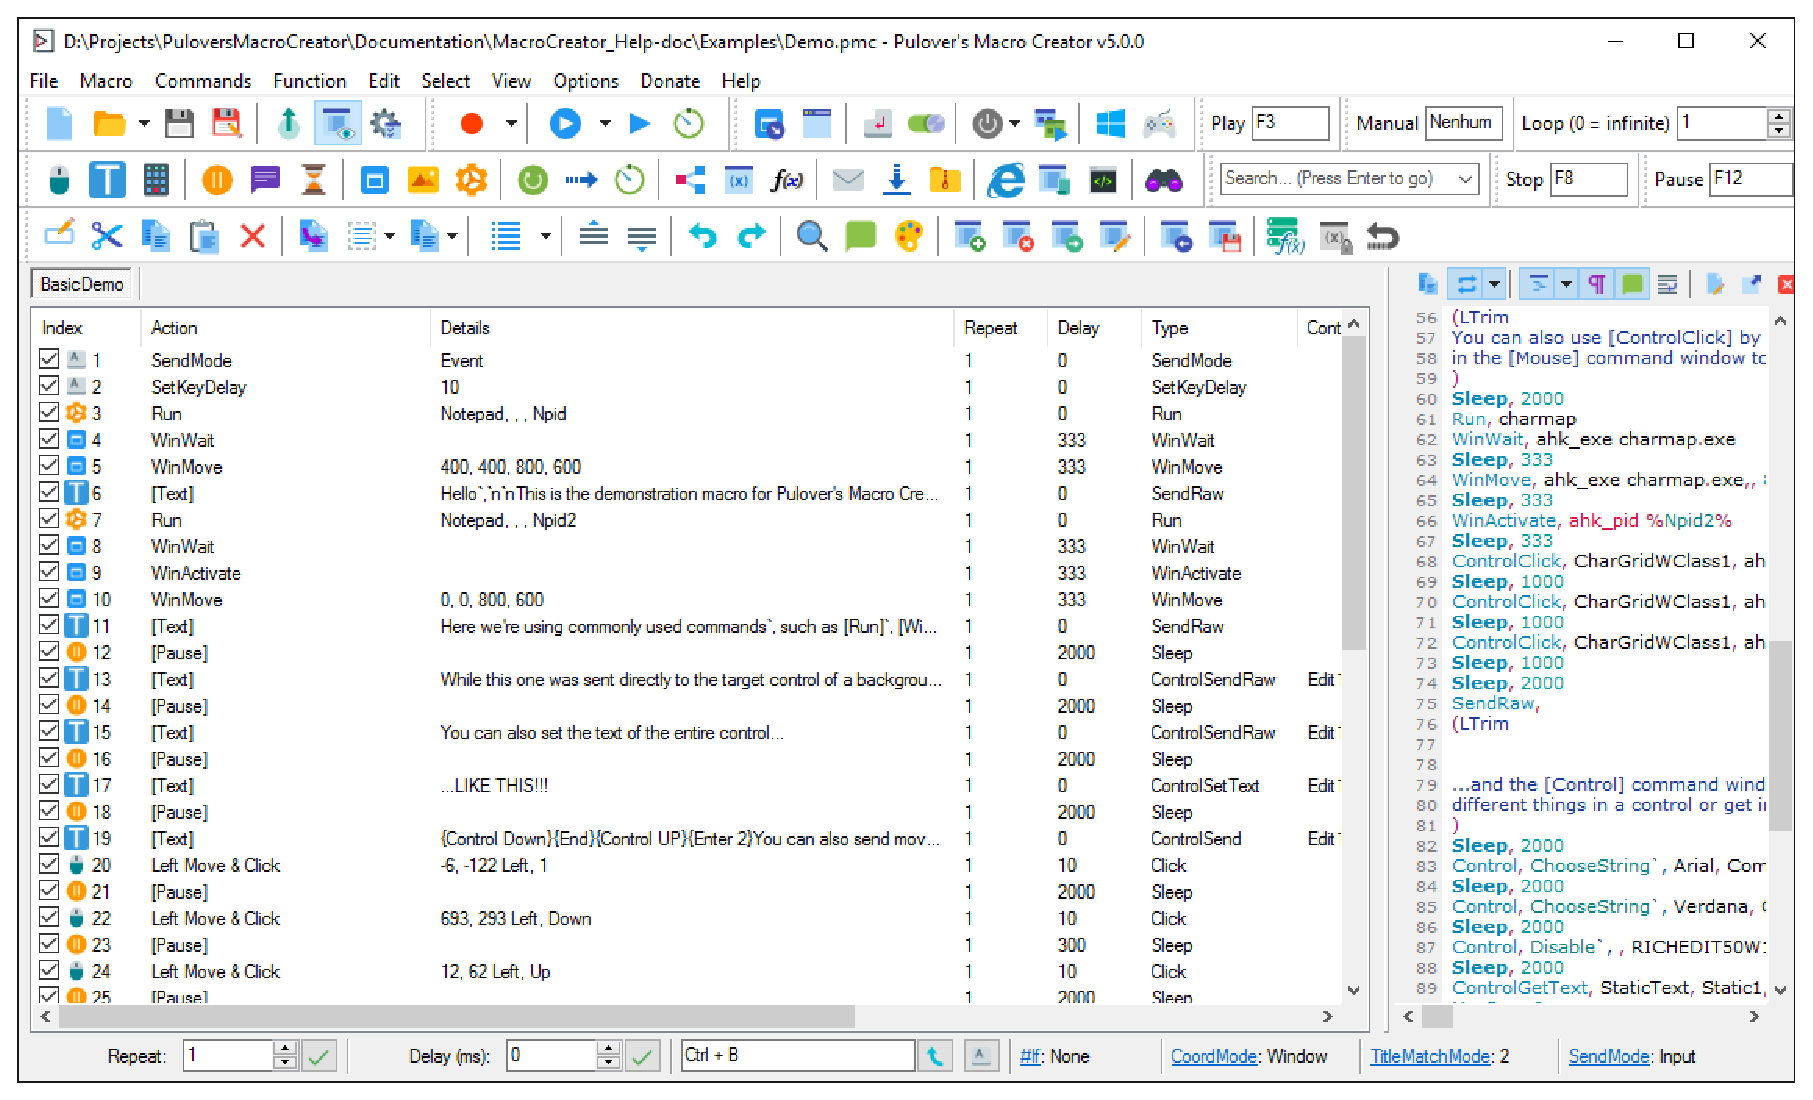
\includegraphics[width=0.7\columnwidth]{chap2/Imagenes/Macros.eps}
\caption{Interfaz de usuario de Pulovers Macro Creator con una macro de
 ejemplo.}
\label{fig:macros}
\end{figure}